\section{Introduction}\label{xs:intro}

\begin{figure}[t]
\centering
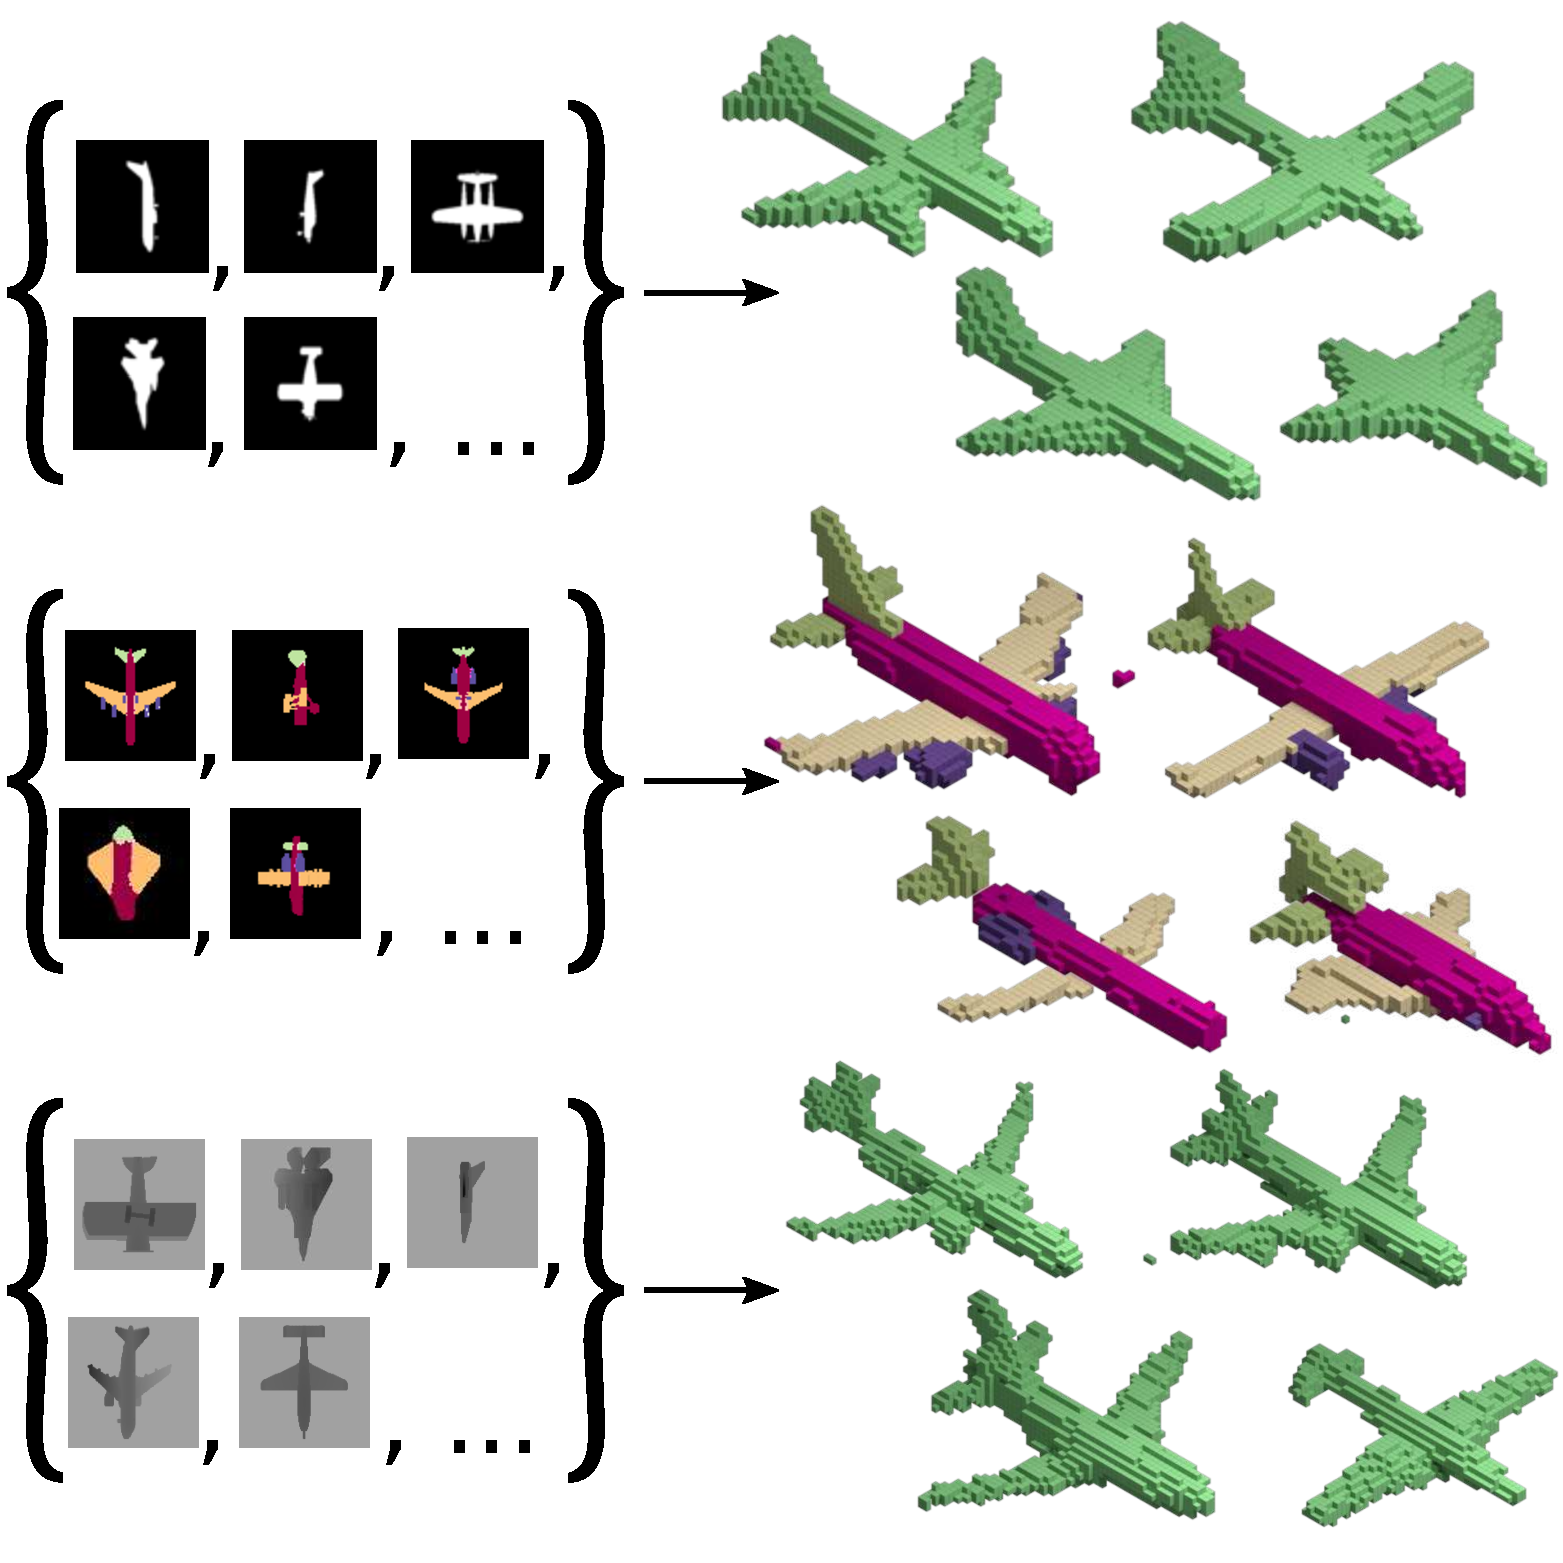
\includegraphics[width=1.0\linewidth]{fig/visabstract.pdf}
\caption{\label{f:problem} Our algorithm infers a generative model of
  the underlying 3D shapes given a collection of unlabeled images rendered as
  silhouettes, semantic segmentations or depth maps. 
	To the left, images representing the input dataset.
	To the right, shapes generated by the generative model trained with those images.}
\vspace{-12pt}
\end{figure}


The ability to infer 3D shapes of objects from their 2D views is one
of the central challenges in computer vision.
For example, when presented with a catalogue of airplane silhouettes
as shown in the top of Figure~\ref{f:problem}, one can mentally infer
their 3D shapes by simultaneously reasoning about the shape and
viewpoint variability.
In this work, we investigate the problem of learning a generative
model of 3D shapes from a collection of images of an unknown set of
objects within a category taken from an unknown set of views.
The images can be thought of as generalized projections of 3D shapes
into a 2D space in the form of silhouettes, depth maps,
or even part segmentations.
The problem is challenging as one is not provided with the information
about which object instance was used to generate each image, the viewpoint from
which each image was taken, the parameterization of the underlying shape
distribution, or even the number of underlying instances.
Hence, traditional techniques based on structure
from motion~\cite{hartley2003multiple,blanz1999morphable} or visual
hulls~\cite{laurentini1994visual}, cannot be directly applied.


We use the framework of generative adversarial
networks (GANs)~\cite{goodfellow2014generative} and augment the 3D shape
generator with a \emph{projection module}, as illustrated in Figure~\ref{fig:prgan-arch}.
The generator produces 3D shapes, the projection module
renders the shape from viewpoint sampled from a viewpoint distribution,
and the adversarial network discriminates real images from generated ones.
The projection module is a \emph{differentiable renderer} that allows us to map 3D
shapes to 2D images, as well as back-propagate the gradients of 2D
images to 3D shapes.
Once trained, the model can be used to infer 3D shape distributions
from a collection of images (Figure~\ref{f:problem} shows some samples
drawn from the generator), and to infer depth or viewpoint from a single
image, without using any 3D or viewpoint information during learning.
We call our approach \emph{projective generative adversarial network}
~(\prgan).








While there are several ways of rendering a 3D shape, we begin with a 
silhouette representation.
The motivation is that silhouettes can be easily
extracted when objects are photographed against clear backgrounds, such
as in catalogue images, but nevertheless they contain rich shape information.
Real-world images can also be used by removing background and converting them to
binary images. 
Our generative 3D model represents shapes using a voxel representation that indicates
the occupancy of a volume in a fixed-resolution 3D grid.
Our projection module is a feed-forward operator that
renders the volume as an image.
The feed-forward operator is differentiable, providing
the ability to adjust the 3D volume based on projections. 
Finally, we assume that the distribution over viewpoints
is known (assumed to be uniform in our experiments, but it could be any
distribution).

We then extend our analysis first presented in our earlier
work~\cite{prgan} by incorporating recent advances in training GANs and
designing projection modules to incorporate richer supervision.
The latter includes the availability of viewpoint information for
each image, depth maps instead of silhouettes, or semantic
segmentations such as part labels during learning.
Such supervision is easier to collect than acquiring full 3D scans of
objects.
For example, one can use a generic object viewpoint
estimator~\cite{su2015render} as weak supervision for our problem.
Similarly, semantic parts can be labeled on images directly and
already exist for many object categories such as airplanes, birds,
faces, and people.
We show that such information can be used to improve 3D reconstruction
by using an appropriate projection module.

To summarize our main contributions are as follows: (i) we propose
\prgan, a framework to learn probabilistic distributions over 3D
shapes from a collection of 2D views of objects. We demonstrate its
effectiveness on learning shape categories
such as chairs, airplanes, and cars sampled from online shape
repositories~\cite{chang2015shapenet,wu20153d}. 
The results are reasonable even when views from multiple categories
are combined; (ii) \prgan generates 3D shapes of comparable quality to GANs trained
directly on 3D data~\cite{wu2016learning};
(iii) The learned 3D representation can be used for unsupervised
estimation of 3D shape and viewpoint given a novel 2D shape, 
and for interpolation between two different shapes, (iv) Incorporating
additional cues as weak supervision improves the 3D shapes
reconstructions in our framework.


